\documentclass[12pt]{article}
\usepackage{graphicx}
\usepackage{multirow}
\usepackage{makeidx}
\usepackage{latexsym}
\usepackage{bm}
\usepackage{amsmath}
\usepackage{amsthm}
\usepackage{amssymb}
\usepackage{setspace}

\usepackage{amssymb}
\usepackage{graphicx}
\usepackage{multirow}
\usepackage{makeidx}
\usepackage{latexsym}
\usepackage{bm}
\usepackage{amsmath}
\usepackage{amsthm}
\usepackage{amssymb}
\usepackage{setspace}

\renewcommand{\rmdefault}{ptm}
%\usepackage[scaled=0.92]{helvet}
\usepackage{courier}
\normalfont 
\usepackage[T1]{fontenc}


%\singlespacing 
\onehalfspacing
%\doublespacing
%\setlength{\textheight}{22.5cm}
%\setlength{\textwidth}{6.47in}
%\setlength{\oddsidemargin}{-1mm}
%\setlength{\topmargin}{0.1cm}
%\setlength{\evensidemargin}{-5mm}

\setlength{\textheight}{24cm}
\setlength{\textwidth}{6.67in}
\setlength{\oddsidemargin}{-5mm}
\setlength{\topmargin}{-1cm}
\setlength{\evensidemargin}{-5mm}

\makeindex

\newcommand{\captionfonts}{\footnotesize}
\makeatletter  
\long\def\@makecaption#1#2{
  \vskip\abovecaptionskip
  \sbox\@tempboxa{{\captionfonts #1: #2}}
  \ifdim \wd\@tempboxa >\hsize
    {\captionfonts #1: #2\par}
  \else
    \hbox to\hsize{\hfil\box\@tempboxa\hfil}
  \fi
  \vskip\belowcaptionskip}
\makeatother

%\renewcommand{\rmdefault}{ptm}


\newcommand {\hide}[1] {\typeout{ #1 }}
\newcommand{\beq}{\begin{equation}}
\newcommand{\eeq}{\end{equation}}
\newcommand{\dif}[2]{\frac{{\rm d} #1}{{\rm d} #2}}
\newcommand{\ildif}[2]{{\rm d} #1/{{\rm d} #2 }}
\newcommand{\ilpdif}[2]{\partial #1/{\partial #2 }}
\newcommand{\pdif}[2]{\frac{\partial #1}{\partial #2}}
\newcommand{\pddif}[3]{\frac{\partial^2 #1}{\partial #2 \partial #3}}
\newcommand{\ilpddif}[3]{\partial^2 #1/{\partial #2 \partial #3}}
\newcommand{\comb}[2]{\left (\begin{array}{c}{#1}\\{#2}\end{array}\right )}
\newcommand{\perm}[2]{^{#1}{\rm P}_{#2}}
\newcommand{\gfrac}[2]{\mbox{$ { \textstyle{ \frac{#1}{#2} }\displaystyle}$}}
\newcommand{\defn}{\begin{quote}{\bf Definition. }}
\newcommand{\edefn}{\end{quote}}
\newcommand{\thm}{\begin{theorem}}
\newcommand{\ethm}{\end{theorem}}
\newcommand{\R}{{\sf R}}
\newcommand{\s}{{\sf S}}
\newcommand{\fnzero}{\setcounter{footnote}{0}}
\newcommand{\bmat}[1]{\left ( \begin{array}{#1}}
\newcommand{\emat}{\end{array}\right )}
\newcommand{\E}{\mathbb{E}}
\newcommand{\ts}{^{\sf T}} 
\newcommand{\its}{^{\sf -T}}
\newcommand{\fv}{\hat{\bm{\mu}}}
\newcommand{\X}{{\bf X}}
\newcommand{\Xt}{\X\ts}
\newcommand{\y}{{\bf y}}
\newcommand{\A}{{\bf A}}
\newcommand{\Qf}{{\bf Q}_{\rm f}}
\newcommand{\bp}{{\bm \beta}}
\newcommand{\rsd}{\hat {\bm \epsilon}}
\newcommand{\grad}{\nabla_\beta}
\newcommand{\tr}[1]{{\rm tr}\left ( {#1} \right )}
\theoremstyle{definition}
\newtheorem*{defin}{Definition}
\theoremstyle{plain}
\newtheorem{theorem}{Theorem}
\newcommand{\rss}{{\cal S}}
\newcommand{\eps}[3]
{{\begin{center}
\rotatebox{#1}{\scalebox{#2}{\includegraphics{#3}}}
\end{center}}
}
\newcommand{\smsz}{\small}


\begin{document}


\title{Modelling the Spatiotemporal Distribution of the Incidence of Resident Foreign Population}

\author{
Giampiero Marra \\ \small Dept of Statistical Science, University College London \\ \small Gower Street, London WC1E 6BT, U.K. 
\\ \small \texttt{giampiero@stats.ucl.ac.uk}
 \and
David L. Miller \\ \small Dept of Mathematical Sciences, University of Bath \\ \small Claverton Down, Bath BA2 7AY, U.K.
 \and
Luca Zanin \\ \small Prometeia \\ \small G. Marconi, Bologna 40122, Italy
}
\date{}

\maketitle


\begin{abstract}

Many European countries have recently experienced a substantial increase in the proportion of immigrants in their populations. The incidence of resident foreigners calculated at a national level does not provide information on the local spatial and temporal distribution of the phenomenon. This information may be of crucial importance for planning local policies. In this paper we suggest a tool for practitioners to provide spatiotemporal maps representing the local distribution of the incidence of resident foreigners in the territory, and changes in spatial trends over time. We illustrate this with Italian data at a municipal level, for the period 2003-2008. To account for spatiotemporal interactions in the data, we propose using a generalized additive model incorporating a smoother of the time and space dimensions. Specifically, we set up a tensor product smoother combining a cubic regression spline basis for time and a soap film spline basis for space. This approach provides a consistent framework to produce spatiotemporal maps which could be effectively used by policy makers to decide the allocation of economic resources at a local level.

\vspace{0.4cm}
\noindent \textbf{Key Words:} Generalized additive model; Incidence of resident foreigners; Soap film spline basis; Spatiotemporal maps; Tensor product smoother. 


\end{abstract}

\section{Introduction \label{IN}}

An increase in both political and academic interest has led to a large amount of research into international migration, both theoretical and empirical, exploring its causes and consequences. Several theories of migration have been proposed, from both a macro- and microeconomic point of view, based on different schools of thought. Among these are the neoclassical economic theory (e.g. Borjas, 1989; Massey \textit{et al.}, 1993), the assumptions regarding the new economics of migration (e.g. Stark and Bloom, 1985; Massey \textit{et al.} 1993), dual labor markets (e.g. Piore, 1979; Massey \textit{et al.} 1993) and world systems theory (e.g. Wallerstein, 1974; Hooghe \textit{et al.} 2008). In addition to theoretical work, many empirical studies have taken place. Examples include studies investigating the impact of resident foreigners on the labor market of the host country (e.g. Borjas, 2003, 2005; Borjas, Freeman and Katz, 1996; Card, 2005; Fullin and Reyneri, 2011), underemployment (Slack and Jensen, 2007), possible connections between immigration and nations' poverty rates (Raphael and Smolensky, 2009), transfer of identity from first to second generation immigrants (Casey and Dustmann, 2010), difference in education, earnings and employment between first and second generation immigrants (Algan \textit{et al.}, 2010), problems relating to the integration of different cultures and languages (e.g. Lazear, 1999; Contucci and Ghirlanda, 2007), and the tendency for immigrants to live in ethnic ``enclaves'' (Edin, Fredriksson and Aslund, 2003). 
  
Manning (2010) has pointed out that many European countries have recently experienced a substantial increase in the proportion of immigrants in the population. Given a specific area such as municipality, province, region or nation, a measure of density of resident foreign population is the percentage incidence of resident foreigners (IRF), given as the ratio of the number of resident foreigners to the total resident population multiplied by 100 (e.g. Lowell, 2007; Coleman, 2008; Miguet, 2008). This gives a simple, well-known, demographic indicator for comparing different regions of a country in terms of number of resident foreigners per 100 resident inhabitants (e.g. OECD, 2004). 

\begin{figure}[tbp]
	\centering
		\includegraphics[width=0.85\textwidth, angle=270]{Raw.ps}
	\caption{Empirical maps of the percentage incidence of resident foreigners in Italy over the years 2003-2008. These were obtained using ISTAT data at a municipal level.	The incidence is given as the ratio of the number of resident foreigners to the total resident population multiplied by 100. The colour scale ranges from an incidence of 0 (dark red) to an incidence of 12 (white).}
	\label{Rd}
\end{figure}

Here we consider the Italian case and aim to analyse the local distribution of the incidence of resident foreigners in the territory. According to the Italian National Statistical Office (ISTAT), the IRF has grown substantially, from 2.7\% in 2002 to 6.5\% in 2008. This phenomenon has had an impact on the population, especially from a socio-demographic point of view (see Section \ref{DEM} for details). The IRF calculated on a national level does not tell us anything specific about the local spatial distribution of the phenomenon. Information on how the distribution of the IRF changes over time and space at a local level (e.g. municipal) may be of crucial importance for planning local policies (e.g. for the integration of resident foreigners in a host country). It is clear that for each municipality the IRF is administrated and known from the municipal population registers. However, for policy makers in the central public administration, geographical maps of the IRF at a municipal level for the whole territory can represent a useful tool providing an overview of the areas with a higher or lower presence of foreigners. In this respect, we would expect, for instance, an area with a high density of resident foreigners to require more economic resources for integration's policies than an area with a lower density.

Our study uses Italian data for the period 2003-2008. Since 2003, ISTAT has provided a new public database with annual frequency of the number of resident foreigners at a municipal level. This represents the current maximum spatial and temporal detail available. Figure \ref{Rd} shows the empirical maps of the IRF at a municipal level over the years 2003-2008. The features that stand out clearly are the marked difference between north and south, and the increase in the IRF over time. However, these maps make it difficult to detect any local spatial structure in the incidence. For example, in the Po Valley (northern Italy), the area is characterized by medium-high IRF levels in 2008 but it is not really possible to identify the existence of any polarization. This can be problematic for policy makers in the central public administration who may want to allocate economic resources as efficiently and effectively as possible. We recall that studies analysing the distribution of resident foreign population in a territory have employed descriptive analysis and/or more or less complex linear modelling approaches (e.g. Ward, 1969; McHugh, 1989; Greenwood and McDowel, 1991; Fonseca, 2008; De Graaff and Nijkamp, 2010; Longhi, Nijkamp and Poot, 2010). Our aim here is to illustrate a tool for practitioners to provide clearer spatiotemporal maps representing the distribution of the IRF in a territory and changes in spatial trends over time, at a local level. 

Common spatiotemporal modelling methodologies include hierarchical Bayesian models, geostatistical models and generalized additive models (e.g. Banerjee, Carlin and Gelfand, 2004; Hastie and Tibshirani, 1990; Kamman and Wand, 2003; Kneib and Fahrmeir, 2006; Osei, Duker and Stein, 2011; Ruppert, Wand and Carroll, 2003; Sahu, Gelfand and Holland, 2007; Wood, 2006). Here we opt for generalized additive models since they allow a wide range of possibilities for representing the model component functions. This is crucial in our case study to fulfill the model requirements, as briefly detailed below. Because currently no relevant economic data are available at a municipal level, the response (IRF) is modelled using a smoother which is a function of only the spatial coordinates and time. The model is then used to create smoothed maps of the geographical area of interest over time. Two points are noteworthy here. First, when a geographical region has complex boundaries, such as Italy for example, a phenomenon known as \textit{leakage} is likely to occur (Ramsay, 2002). In this case, a smoother would inappropriately link two parts of a domain causing the fitted surface to be mis-estimated, leading to incorrect inference (e.g. biased incidence estimates). This issue can be overcome if the smoother used can account for the structure of the domain under investigation; several solutions have been proposed (e.g. Ramsay, 2002; Wood, Bravington and Hedley, 2008, and references therein). Second, because it is unlikely that the IRF occurs at similar strengths and patterns over the territory, the employed approach should account for a space-time interaction. These two goals can be achieved by using a generalized additive model incorporating a scale-invariant three-dimensional tensor product smoother combining a cubic regression spline basis function for the temporal trend and a soap film spline basis for the spatial component (Wood 2006; Wood, Bravington and Hedley, 2008).


\section{The structure and nature of the data on resident foreign population in Italy\label{SDC}}

The entry of foreigners from some countries of the European Union (EU) into Italy is regulated by the Schengen agreements. These allow for the elimination of border controls, hence creating a common area of free movement among members (Broeders, 2007). Foreigners from a non-EU country must possess a visa or the necessary documents (further details are available from the Ministry of the Interior http://www.interno.it). 
 
In studying a phenomenon linked to the international migration, it is important to distinguish between those individuals considered to be resident foreigners and those considered to be immigrants. The resident foreign population includes all people (born in Italy or abroad) who declare their citizenship not to be Italian. The immigrant population consists of all those born abroad who have declared themselves to be foreigners or Italian by naturalization. Foreigners born in Italy such as children born from foreign parents are excluded from immigrant population. The population census conducted by ISTAT in 2001 showed that foreigners and immigrants constitute roughly the same group: about $81\%$ of immigrants have been identified by foreign citizenship, and $88\%$ of foreigners are immigrants (since they were born abroad).

In many countries, official statistics report the number of resident foreigners but not the number of immigrants (Coleman, 2008). Currently, the dynamics of immigration to Italy still allow the acceptance of a definition which does not distinguish between these two groups. This simplification is reasonable during the first phase of the immigration process in a country and when the majority of immigrants keep their own citizenship for a long period. Indeed, this is the case in Italy. The population census gives the best distinction between immigrants and foreigners. In this case the data can be analysed by birthplace, citizenship at birth and citizenship at the census time. 
 
Italian official statistics on the resident foreign population are mainly based on administrative sources. Recently ISTAT has integrated the official statistics with a new public database (http://demo.istat.it). The database gives the number of resident foreigners calculated at the end of December each year in each municipality (of which there are around 8100). Compared to provincial or regional data, municipal-level data offers far more detail on the spatial distribution of the IRF.
 
Populations are of course dynamic over time as well as space. In this regard, the change in resident foreign population at a municipal level, at the end of a year, is determined by
$$
RFP^{31^\text{st}} = RFP^{1^\text{st}} + (I_1 + I_2 + I_3+ I_4) - (D_1 + D_2 + D_3 + D_4 + AC),
$$ 
where $RFP^{31^\text{st}}$ indicates the total number of resident foreigners at the end of December and $RFP^{1^\text{st}}$ the number of resident foreigners on the $1^\text{st}$ of January. $I_{1}$ denotes the number of people whose parents are foreigners (at least one of them being resident in the municipality), $I_{2}$ the number of foreign citizens who asked to transfer their residence from another Italian municipality to the current one, $I_{3}$ those who asked to transfer their residence from abroad, and $I_{4}$ refers to recording operations due to other reasons (e.g. foreigners mistakenly deleted from the registry of the municipality, because they were temporarily missing). $D_{1}$ represents the number of resident foreigners who died during the year, $D_{2}$ those who moved to a different municipality, $D_{3}$ those who moved abroad, $D_{4}$ refers to cancellations for other reasons (e.g. foreigners deleted from the registry of the municipality, because they were not present), and \textit{AC} denotes those resident foreigners who obtained Italian citizenship during the year. 

Acquisition of Italian citizenship by foreigners is regulated by law 91 of the $5^\text{th}$ of February 1992 and its subsequent amendments and additions. Foreigners can acquire Italian citizenship by marriage to an Italian or by naturalization. The latter case refers to the situation in which the foreigner has lived in the country from a certain period of time. Such a period varies dependent on the status of the person in question and the specific laws of each country. For example, in Italy, the period is at least 10 years for non-EU citizens, at least 4 years for EU citizens and at least 5 years for political refugees or stateless persons and adult individuals who have been adopted by Italian citizens. An exhaustive list of ways to obtain Italian citizenship is available on the Ministry of the Interior's website. Once foreigners have acquired Italian citizenship, they are included in the Italian population's statistics. However, our aim is to investigate and measure the incidence on the population of  residents who do not have Italian citizenship.

We do not tackle the issue of illegal foreigners here. This phenomenon and its respective quantification is an open topic of discussion in the studies of international migrations (e.g. Carter, 1999; Hillman and Weiss, 1999; Cangiano, 2008; Strozza, 2004). Several approaches have been proposed in literature to quantify this, but all are subject to criticism (especially with regard to the magnitude of errors in estimates). Here we only consider official data on the resident foreign population. 

\section{The resident foreign population's contribution to Italy's demography \label{DEM}}

Bijak \textit{et al.} (2007) shows that in the absence of migration, many of the 27 European Union countries could see a decline in their non-immigrant populations up to 2052. In particular, with no migration they estimate that the population of Italy could decrease from 57 million in 2002 to about 43 million in 2052. The main causes of this decline may be linked to a low fertility rate and hence an aging population. 

Looking at a traditional indicator of an elderly population, the ratio of old (over 64) to young (up to 14) in the total population was 143.4\% at the end of 2008 (156.2\% if we only consider individuals with Italian citizenship). The elderly population is about $43\%$ larger than the young population. Considering only the resident foreign population the ratio is 11.2\%. In the same year, the average age of foreigners resident in Italy was 31, while that of Italian citizens was 43. From this we can see that if we stratify by citizenship there is a substantial difference in the age structure of the population present in Italy.

As for the low fertility rate, the latest data from ISTAT puts the average number of children per Italian woman of childbearing age (from 15 to 49 years) at 1.33, lower than the average of 2.05 children for foreign woman living in Italy. Combining the fertility rate for both Italian and foreign women, we obtain an average of 1.41. Coleman (2008) states that ``typically, in low-mortality populations a total fertility of about 2.04 is regarded as the `replacement level', that is, a level sufficient to replace the population in the long-run, ignoring migration''. Given the impact of resident foreigners on the population structure, the measure of total fertility (and hence the level of replacement) must take into account the contribution of immigrants (Coleman, 2008). In Italy, the increasing presence of resident foreigners over recent years has contributed not only to population growth but also to a reduction in average age and an increase in the total fertility rate. The profile of the nationalities of resident foreigners in Italy is changing. Based on elaborations of data from ISTAT, in 2003, the top three countries represented were Albania (13.6\%), Morocco (12.7\%) and Romania (8.9\%). In 2008, Romania was top (20.5\%), followed by Albania (11.3\%) and Morocco (10.4\%). The significant increase of the Romanian population in Italy coincides with the country's entry to the European Union ($1^\text{st}$ January 2007). Currently, Romanian is the most numerous foreign nationality in 14 of the 20 Italian regions. Italy hosts the largest Romanian community outside Romania and almost half of the entire Romanian migrant stock. The choice of Italy as primary destination for Romanians can be explained by many factors including the presence of small Italian companies, the economic links with Romania and the accessibility of the Italian language for Romanians (Ban, 2009). 

According to a descriptive analysis of ISTAT data, in 2008 the resident foreign population in Italy was made up of 53.6\% individuals from Europe, 22.4\% from Africa, 15.8\% from Asia, 8.1\% from America, and 0.1\% from Oceania.

\section{Spatiotemporal modelling \label{METH}}

\subsection{Model specification \label{MS}}

The model we employ belongs to the class of generalized additive models (GAMs; Hastie and Tibshirani, 1990). Such models allow for complex relationships between covariates and the response, which can be crucial to uncover interesting features in the data. The IRF can only take positive continuous values. As explained in the introductory section, this is because the IRF used here is given as the ratio of the number of resident foreigners to the total resident population multiplied by 100. The proposed model is as follows
\beq
\text{log}\left\{\E(\texttt{irf}_{it})\right\} = f(\texttt{year}_t,\texttt{n}_i,\texttt{e}_i), \ \texttt{irf}_{it} \sim \text{Tweedie}\left\{\E(\texttt{irf}_{it}),\phi \E(\texttt{irf}_{it})^{p}\right\},          
\label{PropM}
\eeq
at municipality $i=1,\ldots,8094$ and year $t=2003,\ldots,2008$. $\phi$ is a dispersion parameter and the log link function ensures positive fitted values. $\texttt{irf}_{it}$, $\texttt{n}_i$, and $\texttt{e}_i$ represent the variables percentage IRF, Northing and Easting, respectively. Tweedie distributions are a special case of an exponential dispersion model and include, for example, the normal ($p=0$), Poisson ($p=1$) and gamma ($p=2$) distributions (J\o rgensen, 1987). For $1<p<2$ Tweedie distributions can be represented as Poisson mixtures of gamma distributions, with mass at zero but otherwise continuous on the positive reals. These are especially appealing for modelling continuous positive observations when exact zeros occur. Dunn and Smyth (2005) provides a survey of published applications stressing the utility and flexibility of this class of distributions. $f$ is a multidimensional smooth function of \texttt{year}, \texttt{n} and \texttt{e} which models the joint effect of these variables on \texttt{irf}. The use of a three-dimensional smoother for time and space is crucial in that the temporal trend of the IRF is expected to occur at different strengths and patterns depending on the spatial location because of differing site characteristics in the territory. Northing and Easting are simply offsets in kilometres from a set point (in our case, 11.5 longitude, 44 latitude), thus ensuring that the spatial part of the smoother is isotropic (as opposed to using latitude and longitude). We want both the spatial and temporal components to have an optimal degree of smoothness in terms of the bias-variance trade-off; the smoother must be invariant to the relative scaling of space (km) and time (years). In addition, the smoother has to allow for combinations of different basis functions most suitable for the spatial and temporal components. This can be achieved using a multidimensional tensor product smoother combining a cubic regression spline basis for \texttt{year} and a spline basis for the two spatial dimensions \texttt{n} and \texttt{e}. The smooth component in (\ref{PropM}) is subject to some identifiability constraint (see Wood (2006) for more details).

\begin{figure}[tbp]
	\centering
		\includegraphics[width=0.65\textwidth, angle=270]{pointmap.eps}
	\caption{Raw data locations for the incidence of resident foreigners with the boundaries of Italy, Sardinia and Sicily. Each point is the location of the centroid of a municipality.}
	\label{pointmap}
\end{figure}

Note that the data used here are collected per municipality but enter into the model as points which are located at the centroids of the municipalities (see Figure \ref{pointmap}). This change of support from areal to point data is not problematic and is desirable. In fact, our aim is to produce smoothed maps; using areal data would yield maps that are step functions for each municipality hence making it more difficult to see patterns in the data. Since we endeavour to make the maps as easily interpretable as possible, smoothing of points is a clear choice.

The next two sections cover the technical details of the construction of the smoothers. We first show how in general a three-dimensional tensor product smoother can be constructed using a one-dimensional temporal smoother and a two-dimensional spatial smoother. We then go into the details of the construction of the two-dimensional smoother.

\subsection{A three-dimensional tensor product smoother for time and space \label{3D}}

The construction of a three-dimensional scale invariant tensor product smoother of time and space is based on a marginal one-dimensional spline basis for time and a two-dimensional marginal smooth function for space, with associated quadratic penalties measuring their roughness. We omit the subscripts $i$ and $t$ for simplicity. Let us assume that we have two low-rank regression spline bases of any type to represent the smooth functions $f_\text{year}$ and $f_\text{space}$, we can write
$$
f_\text{year}(\texttt{year})=\sum_{l=1}^L \xi_l b_l(\texttt{year})=\textbf{X}_\text{year}\bm\xi \ \ \text{and} \ \ f_\text{space}(\texttt{n},\texttt{e})=\sum_{r=1}^R \varphi_r d_r(\texttt{n},\texttt{e})=\textbf{X}_\text{space}\bm\varphi,
$$
where the $b_l(\texttt{year})$ and $d_r(\texttt{n},\texttt{e})$ are known cubic regression spline and soap film basis functions, with corresponding parameters $\xi_l$ and $\varphi_r$ and spline dimensions $L$ and $R$. $\textbf{X}_\text{year}$ and $\textbf{X}_\text{space}$ are marginal model matrices evaluating the basis functions with parameter vectors $\bm\xi$ and $\bm\varphi$. The expansion for $f_\text{space}$ and its roughness penalty do not correspond exactly to the expressions used to set up the model since, in this section, we are concerned with illustrating the construction of a three-dimensional scale invariant tensor product smoother. It is therefore convenient to keep the description of the two-dimensional marginal smoother for space and its quadratic penalty as simple as possible; a rigorous description will be given in the next section. 

In order to set up a three-dimensional tensor product smoother for time and space we need $f_\text{year}(\texttt{year})$ to vary smoothly within the space dimensions. This can be achieved by allowing the parameters $\xi_l$ to vary smoothly with \texttt{n} and \texttt{e}. Using the spline set-up for $f_\text{space}(\texttt{n},\texttt{e})$ we may write (e.g. Wood, 2006, p. 163)
$$
\xi_l(\texttt{n},\texttt{e})=\sum_{r=1}^R \varphi_{lr} d_r(\texttt{n},\texttt{e})
$$    
which results in
$$
f(\texttt{year},\texttt{n},\texttt{e})=\sum_{l=1}^L \sum_{r=1}^R \varphi_{lr} d_r(\texttt{n},\texttt{e}) b_l(\texttt{year}). 
$$
For any particular set of observations of \texttt{year}, \texttt{n} and \texttt{e}, there exists a simple relationship between the matrix $\textbf{X}$ evaluating the tensor product smoother at these observations and the model matrices $\textbf{X}_\text{year}$ and $\textbf{X}_\text{space}$ evaluating the marginal smooths at the same observations. Ordering appropriately the parameters $\varphi_{lr}$ into a vector $\bm\theta$, the $i^{th}$ row of $\textbf{X}$ is given by $\textbf{X}_{i}=\textbf{X}_{\text{year},i}\otimes\textbf{X}_{\text{space},i}$, where $\otimes$ is the Kronecker product. 

In the GAM context, it is necessary to quantify the roughness of the smooth functions in the model so that over-fitting can be accounted for and hence avoided during the parameter estimation process (e.g. Marra and Radice, 2010). As for the penalty associated with this tensor product basis, it is possible to start from roughness measures associated with the marginal smooths $f_\text{year}(\texttt{year})$ and $f_\text{space}(\texttt{n},\texttt{e})$. Suppose that functionals $J$ measuring the roughness of the smooth terms are available, and that these can be written as quadratic forms in the marginal parameters, we have that
$$
J_\text{year}(f_\text{year})=\bm\xi\ts\textbf{S}_\text{year}\bm\xi \ \ \text{and} \ \ J_\text{space}(f_\text{space})=\bm\varphi\ts\textbf{S}_\text{space}\bm\varphi,
$$
where the $\textbf{S}$ matrices contain known coefficients whose values depend on the chosen bases for time and space. For instance, the second-order cubic spline penalty for $f_\text{year}(\texttt{year})$ evaluates $J_\text{year}(f_\text{year})=\int\left( \partial^2 f_\text{year}/\partial \texttt{year}^2 \right)^2 \text{d}\texttt{year}$, but it may be more complex. An overall penalty for the tensor product smoother can be obtained by applying the penalties of $f_\text{space}(\texttt{n},\texttt{e})$ to the varying coefficients of the marginal smooth $f_\text{year}(\texttt{year})$, $\xi_l(\texttt{n},\texttt{e})$,
$$
\sum_{l=1}^L J_\text{space}\left\{  \xi_l(\texttt{n},\texttt{e}) \right\},
$$ 
and the penalties of $f_\text{year}(\texttt{year})$ to the varying coefficients of the marginal smooth $f_\text{space}(\texttt{n},\texttt{e})$, $\varphi_r(\texttt{year})$,  
$$
\sum_{r=1}^R J_\text{year}\left\{  \varphi_r(\texttt{year}) \right\}.
$$ 
It follows that the roughness penalty of $f(\texttt{year},\texttt{n},\texttt{e})$ can be measured as 
$$
\lambda_\text{space} \sum_{l=1}^L J_\text{space}\left\{  \xi_l(\texttt{n},\texttt{e}) \right\} + \lambda_\text{year} \sum_{r=1}^R J_\text{year}\left\{  \varphi_r(\texttt{year}) \right\},
$$
which can also be written as
\beq
\lambda_\text{space} \bm\theta\ts \textbf{I}_L \otimes \textbf{S}_\text{space} \bm\theta + \lambda_\text{year} \bm\theta\ts \textbf{S}_\text{year} \otimes \textbf{I}_R  \bm\theta,
\label{TensProd}
\eeq
where, once again, the vector $\bm\theta$ contains the tensor product smooth parameters. The $\lambda$ are smoothing parameters controlling the trade-off between model fit and model smoothness. The next section shows how $f_\text{space}$ and $\textbf{S}_\text{space}$ can be constructed.   

Expression (\ref{TensProd}) gives the tensor product penalty in the most general terms. However, in order to have an expression which can be later related to the spatial smoother described in the next section, we re-express the penalty as
$$
\bm\theta\ts \textbf{I}_L \otimes \textbf{S}^*_\text{space} \bm\theta + \bm\theta\ts \textbf{S}^*_\text{year} \otimes \textbf{I}_R  \bm\theta,
$$
where $\textbf{S}^*_\text{space}=\lambda_\text{space} \textbf{S}_\text{space}$ and $\textbf{S}^*_\text{year}=\lambda_\text{year} \textbf{S}_\text{year}$.


\subsubsection{Soap film \label{SF}}

As alluded to in the introduction, the smoother used for the spatial part of the model must take into account of the fact that the borders of Italy represent both physical and administrative boundaries. Clearly a simple spatial smoother would smooth over the bounding box encompassing all of the region we wish to draw inference on. This is not useful; first, because there are no resident foreigners in the sea (at best there are merely potential resident foreigners) and second, because smoothing over this whole area could cause leakage, as mentioned in the introduction.

Leakage occurs when a smoother inappropriately links two parts of a domain. This can happen when a two peninsulae jut out into the sea with different population densities on either side. Say one side has a very high density, whereas the other is significantly lower. Most smoothers will not respect that the two areas are different and should be treated so. Rather, the model will ``smooth across'' this gap, causing the high functional values to ``leak'' into the low valued peninsula and vice versa. There are, of course, situations in which leakage is appropriate. For example, in a study of the propagation of a chemical through a river system, there are several mechanisms to transport the chemical (e.g. surface water flow, animals) other than the river itself. Therefore, there must be a motivation for why we wish to use a model that specifically prevents leakage. This is the case here, as there is no particular reason we should believe that the resident foreign population should be continuous across physical boundaries such as the Mediterranean Sea. Although there is no reason \textit{a priori} to believe that there will be particularly troublesome leakage in our study, we believe that mitigating against the issue by use of appropriate basis function choice is the most sensible course of action. 

The soap film smoother uses a rather simple physical model to prevent leakage from occurring (Wood, Bravington and Hedley, 2008). First, consider the domain boundary to be made of wire, then dip this wire into a bucket of soapy water; you will have a soap film with the same shape as the boundary. Now consider the wire to lie in the $\texttt{n}$-$\texttt{e}$ plane and the height of the soap film at a given point to be the functional value of the model. This film is then distorted smoothly by moving it vertically toward each datum locally, while minimizing the surface tension in the film as a whole. Mathematically, the domain ($\Omega$) is bounded by some polygon ($B$) which, in this case, is the coastlines.

In order to perform soap film smoothing, we must first construct two sets of basis functions to form a smoother that conforms to the necessary boundary conditions. The first basis is used for the smoothing within the region of interest ($\Omega$); the second is for finding the values on the boundary (i.e. smoothing on $B$ itself). These bases are then summed to form
$$
f_\text{space}(\texttt{n},\texttt{e})=\sum_{j=1}^J \alpha_j a_j(\texttt{n},\texttt{e}) + \sum_{k=1}^K \gamma_k g_k(\texttt{n},\texttt{e}),
$$
where the $\gamma_k$ and $\alpha_j$ are the parameters to be estimated. One can think of the $a_j(\texttt{n},\texttt{e})$ as an offset dictated by the estimated boundary conditions on $B$ (although it is important to note that they are not planes) and the sum of the $g_k(\texttt{n},\texttt{e})$ as the smooth function to the data inside $\Omega$. For convenience later, we label the second sum as $f_\text{int}$. We now show how these bases are constructed.

For the internal part of the smoother we first find a set of functions $\rho_k(\texttt{n},\texttt{e})$. These are each solutions to the Laplace's equation in two dimensions
$$
\frac{\partial^2\rho}{\partial \texttt{n}^2} + \frac{\partial^2\rho}{\partial \texttt{e}^2} = 0,
$$
except at one of the knots ($\texttt{n}^*_k,\texttt{e}^*_k$). Then, we solve Poisson's equation in 2-dimensions
\beq
\frac{\partial^2 g_k}{\partial \texttt{n}^2} + \frac{\partial^2 g_k}{\partial \texttt{e}^2} = \rho_k(\texttt{n},\texttt{e}),
\label{soap-poisson}
\eeq
for $k$ indexing the $K$ knots. When the boundary condition $\rho_k(\texttt{n},\texttt{e})=0$ is applied, the set of basis functions for the soap film smoother $g_k(\texttt{n},\texttt{e})$ are found.  The partial differential equations (PDEs) are solved numerically using successive over-relaxation (see the appendix of Wood, Bravington and Hedley (2008) for further details).

To find the boundary basis we first take a `boundary function', $f_\text{bnd}(r)$, using cyclic splines. The function evaluates the height of the function at each point around the boundary. $f_\text{bnd}(r)$ will have the expansion
\beq
f_\text{bnd}(r)=\sum_{j=1}^J \alpha_j \delta_j(r),
\label{soap-cyclic}
\eeq
where $r$ is the distance along the boundary, the $\alpha_j$ are parameters and $\delta_j(r)$ are known cubic spline basis functions. To ensure that the spline is cyclic the usual constraint is enforced: the value of the function at the first knot is the same as that at the last knot up to their second derivatives. Note that we do not find the $\alpha_j$ at this stage, for now we are only interested in the expansion. The basis functions $a_j(\texttt{n},\texttt{e})$ themselves can be found by solving (\ref{soap-poisson}) for $\rho_k(\texttt{n},\texttt{e})= 0$ with the boundary condition resulting from setting $\alpha_j=1$ (and all other $\alpha_i$ to zero) in (\ref{soap-cyclic}), using the same methods as for the $g_k(\texttt{n},\texttt{e})$ above. The $a_j(\texttt{n},\texttt{e})$ can be thought of as the set of functions with a peak at each of the $J$ points around the boundary which in turn are smooth across the whole of $\Omega$.

We have now found the set of basis functions for the inside of the domain and also the boundary-induced-smooth which acts as a base for the soap film smoother. Although this seems like a rather esoteric setup, all the procedure above is effectively doing is setting up a basis in order that we can use standard penalized regression techniques. Just as we might choose one spline basis over another for some property it possesses, the soap film basis has the property that it obeys the (estimated) boundary conditions of the region we are smoothing over.

As with the basis, the penalty is split into two parts: one for the cyclic smoother around the boundary and the other for the internal smoother. Writing $\bm\beta$ as the vector of all smooth coefficients for the soap film, $\bm\gamma$ for the boundary parameters and $\bm\alpha$ for the interior, we have
$$
\bm\beta^\text{T}\textbf{S}^*_\text{space}\bm{\beta} = \lambda_\text{bnd} \bm\gamma^\text{T}\textbf{S}_\text{bnd}\bm{\gamma} + \lambda_\text{int} \bm{\alpha}^\text{T}\textbf{S}_\text{int}\bm{\alpha},
$$
where 
$$
\textbf{S}^*_\text{space} = \lambda_\text{bnd} \textbf{S}_\text{bnd} + \lambda_\text{int} \textbf{S}_\text{int}.
$$
$\textbf{S}^*_\text{space}$ is the total penalty for the spatial part of the smoother, $\textbf{S}_\text{int}$ is the interior penalty and $\textbf{S}_\text{bnd}$ is the cyclic spline boundary penalty. Both are matrices of known coefficients depending on the chosen basis functions. The $\lambda$ are the smoothing parameters for the boundary and interior smooth terms respectively. As in the previous section, for mathematical convenience, an asterisk indicates that the penalty matrices have been multiplied by the appropriate smoothing parameters. We now look at the two parts of the penalty individually. 

The isotropic interior penalty term is calculated as
$$
\textbf{S}_\text{int} = \int_\Omega \Big(\frac{\partial^2 f_\text{int}}{\partial \texttt{n}^2}+\frac{\partial^2 f_\text{int}}{\partial \texttt{e}^2} 
\Big)^2\text{d}\texttt{n}\text{d}\texttt{e}.
$$
Note that the integration occurs only over $\Omega$ rather than over the whole of $\mathbb{R}^2$ as would usually be the case. Also, there is no mixed derivative term, and the whole integrand is squared rather than each term individually (in contrast with, say, a thin plate regression spline). This allows the $\texttt{n}$ and $\texttt{e}$ terms' derivatives to be traded off against each other so that the nullspace of the penalty is infinite dimensional. This permits those functions in the nullspace to be sufficiently wiggly to meet any boundary conditions. The penalty for the cyclic spline running about the boundary, used to estimate the $\alpha_j$, is calculated as (e.g. Wood, 2006)
$$
\textbf{S}_\text{bnd} = \int_B \Big(\frac{\partial^2 f_\text{bnd}}{\partial r^2}\Big)^2 \text{d}r.
$$

The solution of the PDEs above, yielding the basis and penalty, is the most computationally expensive part of the procedure. Knots to use for $\texttt{n}_k^*$ and $\texttt{e}_k^*$ must be specified; here we use a grid (further detail on our exact setup is given in Section \ref{ER}). In summary, we now have both the basis functions $a_j(\texttt{n}_i,\texttt{e}_i)$ and $g_j(\texttt{n}_i,\texttt{e}_i)$, and the penalties $\textbf{S}_\text{bnd}$ and $\textbf{S}_\text{int}$, forming $\textbf{S}^*_\text{space}$, for the soap film smoother. Soap basis functions and penalties can be obtained using the the \texttt{R} package \texttt{soap} which implements the ideas discussed in this section.

The smooth function for $f_\texttt{space}$ obtained using the construction outlined above is rotationally invariant. Two smoothing parameters are estimated for the soap film (one for the interior and one for the boundary) but each controls the smoothness for both geographical directions at once (Wood, Bravington and Hedley, 2008). However, the tensor product smoother using the cubic regression spline basis for time and a soap film for space is not isotropic in space-time. This anisotropy is desirable since, as explained in Section \ref{MS}, the measurements of space and time are on different scales so it would not make sense to estimate one smoothing parameter for both the spatial and temporal components (e.g. Wood, 2006, p. 162).


\subsection{Parameter estimation \label{PE}}

In model (\ref{PropM}), replacing $f$ with its tensor product expression yields a generalized linear model (GLM; McCullagh and Nelder, 1989) whose design matrix contains the spline bases representing the smooth component in the model. In principle such a model can simply be estimated by maximum likelihood (ML). However, in a smoothing spline context, unpenalized parameter estimation is likely to result in smooth component estimates that are too `wiggly', hence undermining the utility of such a model. This can be overcome by penalized ML, where the use of penalties allows for the suppression of that part of smooth term complexity which has no support from the data (e.g. Marra and Radice, 2010). Specifically, the model can be fitted by minimisation of
\beq
D(\bm\theta) + \bm\theta\ts\textbf{S}^*\bm\theta \ \  \text{w.r.t.} \ \  \bm\theta,
\label{Dev}
\eeq
where $\bm\theta$ contains all tensor product parameters associated with the one-dimensional spline basis for time and two-dimensional smoother for space, and $\textbf{S}^*=\sum_i \lambda_i \textbf{S}_i$, where the $\textbf{S}_i$ are matrices of known coefficients properly defined according to the results of the previous sections. The $\lambda_i$ are smoothing parameters. The model deviance, $D$, is defined as $2\phi(l_{\text{sat}}-l)$, where $\phi$ is a dispersion parameter, $l$ is the log-likelihood of the model and $l_{\text{sat}}$ the maximum value for the log-likelihood of the model with one parameter per datum. 

Given values for the $\lambda_i$, minimisation of (\ref{Dev}) is straightforward. However, smoothing parameter estimation has to be addressed. This can be achieved by minimisation of a prediction error estimate, such as the generalized cross-validation (GCV) (Craven and Wahba, 1979), or by approximate restricted ML (REML) estimation (Wood, 2011). Smoothing parameter selection via the GCV consists of minimizing 
\beq
V(\bm\lambda)=\frac{nD(\hat{\bm\theta})}{\left\{n-\text{tr}(\textbf{F})\right\}^2},
\label{GCV1}
\eeq
where $n$ is the sample size, $\textbf{F}$ the usual hat matrix, and $\text{tr}(\textbf{F})$ represents the effective degrees of freedom of the penalized model. Wood (2006) described a computational procedure to estimate smoothing parameters on the basis of criterion (\ref{GCV1}). As an alternative, approximate REML can be employed. Within this framework, the penalized likelihood estimates, $\hat{\bm\theta}$, can be seen as the posterior modes of the distribution of $\bm\theta|{\bf y}$ if $\bm\theta \sim \mathcal{N}(\textbf{0},\textbf{S}^{*-1}\phi)$, where $\textbf{S}^{*-1}$ is an appropriate generalized inverse. Viewing the spline parameters as random effects allows for the possibility to estimate the $\lambda_i$ via REML (Wahba, 1985). The recent work by Reiss and Ogden (2009) shows that at finite sample sizes GCV is prone to under-smoothing and is more likely to develop multiple minima than REML. Furthermore, it is well known that smoothing methods based on prediction error criteria, such as (\ref{GCV1}), are more affected by the presence of correlated errors than maximum likelihood-based smoothing procedures, such as REML (e.g. Krivobokova and Kauermann, 2007). Given the arguments above we opt for approximate REML, and use the \texttt{R} package \texttt{mgcv} for smoothing parameter selection (Wood, 2011). 

\subsection{Variance and trend estimation \label{VE}}

Taking a Bayesian view we can construct intervals using the posterior distribution of the model parameters. This approach was originally proposed by Wahba (1983) or Silverman (1985) in the univariate spline model context, and then generalized to the component-wise case when dealing with Gaussian and non-Gaussian data (e.g. Gu and Wahba, 1993; Ruppert, Wand and Carroll, 2003). The interesting feature of these intervals is that, since they include both a bias and a variance component, they have good observed \textit{frequentist} coverage probabilities across the function (Nychka, 1988; Marra and Wood, in press). The posterior distribution is given as
\beq
\bm\theta|{\bf y} \dot{\backsim} \mathcal{N}( \hat{\bm\theta}, {\bf V}_{\bm\theta} ),
\label{Poster}
\eeq
where $\hat{\bm\theta}$ is the maximum penalized likelihood estimate of $\bm\theta$, which is of the form $(\X\ts{\bf W}\X+{\bf S}^*)^{-1}\X\ts{\bf W}{\bf z}$, ${\bf V}_{\bm\theta} = (\X\ts{\bf W}\X+{\bf S}^*)^{-1}\phi$, $\X$ contains the columns associated with the regression spline bases used to set up the model, and ${\bf W}$ and $\mathbf{z}$ are the diagonal weight matrix and the pseudodata vector at convergence of the algorithm used to fit the penalized model (e.g. Wood, 2006, 2011). Given result (\ref{Poster}), it is easy to find confidence intervals for linear functions of the parameters such as smooth components. Intervals for non-linear functions of the model coefficients can be conveniently obtained by simulation from the posterior distribution of $\bm\theta$. Result (\ref{Poster}) can also be used to produce trend estimates as discussed next.

To aid interpretation of the results, trend estimates for some given areas of interest can be produced using the predictive distribution of $\texttt{irf}_{it}$, constructed employing the result of the previous paragraph. This approach can be implemented as follows:

\begin{enumerate}
	\item Repeat the following steps for $b=1,\ldots,N_b$, where $N_b$ represents the number of random draws. 
	   \begin{enumerate}
	      \item Simulate a random $\mathcal{N}(\hat{\bm\theta}, \hat{{\bf V}}_{\bm\theta} )$ and call the resulting coefficient vector $\bm\theta_b$.
	      \item Calculate $\widehat{\E(\texttt{irf}_{it})}=\widehat{\texttt{irf}}_{itb}=\exp(\X^*_{it}\bm\theta_b)$, where $\X^*_{it}$ is evaluated at the observed values. 
	      \item For a given area of interest $a$ and year $t$, calculate
	      $$\widehat{\overline{\texttt{irf}}}_{tb}^a=\frac{1}{n_a}\sum_{i=1}^{n_a} \widehat{\texttt{irf}}_{itb},$$
	      where $n_a$ represents the number of observations in area $a$.     
	   \end{enumerate}
	\item Produce the required summary statistics, in this case median, lower and upper $95\%$ quantiles, for the temporal trend $\widehat{\overline{\texttt{irf}}}_{tb}^a$.
\end{enumerate}
Small values for $N_b$ are typically tolerable. In practice, $N_b$ can be set to $100$. Increasing this value does not change the results which are presented in the next section.
 

\section{Estimation results \label{ER}}

The model was implemented using the basis sizes (for the cubic and cyclic regression splines) and interior knots (for the soap film) given in Table \ref{soap-basis-table}. Note that separate models were used for each of main land, Sicily and Sardinia since the numerical routine used does not currently support tensor product smoothers with multiple penalties. 

\begin{table}[htbp]
\centering
\begin{tabular}{c c c c}\\
\hline
\hline
Region & Interior knots & Cyclic spline basis size & Cubic spline basis size\\
\hline
Main land & 41 (14x14) & 20 & 6\\
Sardinia & 12 (5x6) & 8 & 6\\
Sicily & 12 (6x6) & 10 & 6\\
\hline
\hline
\end{tabular}
\caption{Basis sizes per region for the smooth functions to be fit to the Italian data. For the interior (soap film) knots, the numbers in brackets show the initial grid, the other number gives the number of knots actually used (those inside the boundary).}
\label{soap-basis-table}
\end{table}

The parameter $p$ in (\ref{PropM}) was set to $1.2$. It was chosen by trial and error to produce the best possible residual plots. The estimate for $\phi$ was equal to $0.905$. Before employing the class of Tweedie models, we used the simpler gamma distribution; diagnostic plots suggested the presence of substantial structure in the residuals. Residual analysis was carried out following an approach similar to that of Chandler (2005). Figure \ref{Resid} gives some diagnostics for the proposed model. Overall, the first two sets of boxplots do not show long-term trends, but suggest the presence of some spatial residual structure. The normal Q-Q plot shows some curvature in the upper tail. The scale-location plot indicates the presence of some heteroscedasticity, although the LOESS smoothed estimate does not indicate a relationship between absolute residuals and predicted values. The presence of extreme values in all diagnostic plots suggest under-estimation of the IRF on occasion. Descriptive analysis revealed that some municipalities register considerably higher IRF levels as compared to those registered in neighboring municipalities. This is mainly due to the specific socio-economic features of attractiveness of each municipality which need to be accounted for in order to avoid under-estimation. Unfortunately, as pointed out in the introduction, currently no relevant economic data are available at a municipal level and hence such information can not be incorporated in the model. The deviance explained was 57\%. 

Because the presence of the moderate spatial residual structure highlighted in Figure \ref{Resid}  might have had a detrimental impact on the final smoothed maps, we attempted to employ a generalized additive mixed model (GAMM; Lin and Zhang, 1999), which can handle smooth function estimation and a number of error correlation structures simultaneously. Since a GAMM can be seen as a generalized linear mixed model, estimation can be achieved using, for instance, penalized quasi-likelihood (Breslow and Clayton, 1993). We used \texttt{mgcv}, which iteratively calls the \texttt{lme()} function of the \texttt{nlme} package for maximization (Pinheiro \textit{et al.} 2009). No models could be fitted due to convergence failures (see Ruppert, Wand and Carroll (2003) and Wood (2006) for problems and limitations with this approach). Alternatively, we tried a fixed effect approach (e.g. Wooldridge, 2002) but there was no significant change in the spatiotemporal maps of the IRF. As a last check, we fitted the proposed model but replacing the response variable with the deviance residuals and suppressing the intercept. The resulting maps suggested the presence of some residual structure in those municipalities characterized by very high IRF levels; this was expected given the presence of extreme residuals evidenced in the diagnostic plots. Finally, sensitivity analysis showed that the results do not change if we use more basis functions for the smooth term in the model. This supports the theoretical result that REML smoothing parameter selection may not be sensitive to moderate misspecifications of the correlation structure (e.g. Krivobokova and Kauermann, 2007). 

\begin{figure}[tbp]
	\centering
		\includegraphics[width=0.75\textwidth, angle=270]{Resid.eps}
	\caption{Deviance residual diagnostics from the final model. Row-wise from top: (i) yearly distributions, (ii) distributions of residuals grouped according to squares on a 10x10 grid which fell inside the boundary, (iii) normal Q-Q plot, (iv) absolute residuals versus predicted values, with LOESS curve (grey line).}
	\label{Resid}
\end{figure}

Using the classic Schwarz's Bayesian criterion (SBC), we compared the proposed model with one in which the spatial effect was assumed to be additive in time; the latter yielded an increased SBC. We also compared the results obtained under the two cases. As compared to the results obtained using the proposed model (see next section), the model not accounting for a space-time interaction produced maps whose certain key features/trends could not be revealed. 

Despite the lack of fit corresponding to those municipalities characterized by very high levels of the IRF, the analysis above suggests that the proposed model is able to capture the overall spatiotemporal structure present in the data. Should some relevant economic variables become available at a municipal level, the model specification and, as a consequence, its explanatory power could be considerably improved. 

\subsection{Spatiotemporal maps \label{STT}}

As mentioned in the introductory section, Italy's national IRF was 6.5\% in 2008. Obviously, this number tells us nothing about specific local areas with particularly high or low levels of resident foreigners. As we move to smaller aggregations (e.g. regional or provincial level) the same argument holds: some information is lost. This kind of low resolution statistic can mask smaller-scale heterogeneity in the population. Our aim here is to capture exactly this spatial heterogeneity.

At first glance, Figure \ref{Rd} shows the stark contrast between north and south. The maps also highlight the inhomogeneous spatial and temporal distribution of the IRF. However, as pointed out in the introduction, smoothed maps can give a much better picture of the distribution of the IRF. Smoothing the maps allows us to both separate out the signal and noise in the data, giving a an idea of the overall structure of the phenomena, as well as providing a trend information via a temporal component of the model. Figure \ref{fig1} shows smoothed spatiotemporal maps of the IRF in Italy for the period 2003-2008, obtained using the approach described in the previous sections. We can see that in 2003 northern and central Italy have the highest levels IRF. Over the subsequent years (2004-2008), the incidence spreads, forming four main areas where resident foreigners tend to live. Focusing on 2008, the most popular areas are in north Italy, specifically the Emilia-Romagna and Lombardy regions. These, although popular in 2003, appear to have greatly expanded. The second most attractive area is made up of the central Italian regions of Tuscany, Umbria, Marche and Lazio. The final two areas are composed of Liguria and Piedmont, and Veneto, Friuli-Venezia Giulia and Trentino-Alto Adige. These are located in the northwest and northeast of the country, respectively. There is also an interesting growth in the incidence at the Swiss and Austrian borders (from about 2\% in 2003 to about 4-5\% in 2008). Resident foreigners seem less attracted by the regions and islands of southern Italy. Returning to the Po Valley, the maps in Figure \ref{fig1} allow us to identify the presence of two large, well defined polarization patterns in the IRF, the first in the centre of the Po Valley and the second near Venice. The maps in Figure \ref{Rd} do not reveal these patterns.

\begin{figure}[tbp]
	\centering
		\includegraphics[width=0.85\textwidth, angle=270]{maps-Soap.ps}
	\caption{Spatiotemporal maps of the percentage incidence of resident foreigners in Italy over the years 2003-2008. These were obtained using model (\ref{PropM}) with a tensor product smoother based on a cubic regression spline basis for time and a soap film spline basis for space, and ISTAT data at a municipal level. Predictions were made over those points lying inside the study region from a 100 by 100 grid. The incidence is given as the ratio of the number of resident foreigners to the total resident population multiplied by 100. The colour scale ranges from an incidence of 0 (dark red) to an incidence of 12 (white). Blue lines indicate contours separated by a one unit change in incidence.}
	\label{fig1}
\end{figure}

Figure \ref{trends} shows the estimated temporal trends for both the full Italian territory and broken down by area with 95\% confidence intervals. The trends for northern and central Italy are similar. However, those for southern Italy and the islands are much flatter. Northern and central Italy also show a faster growth in incidence. Such differences are supported by the confidence intervals. Overall, these trends reflect what we see in the maps in Figure \ref{fig1}, that there is a significant difference between northern/central Italy and the south of the country and its islands. Note that, since the approach outlined in Section \ref{VE} can not account for the presence of residual correlation structure, we expect the obtained confidence intervals not to be exactly representative than those that might be produced using some adjusted version of them. The most obvious approach would be to fit a GAMM with a carefully chosen correlation structure and use the resulting posterior covariance matrix in place of that reported in Section \ref{VE}. Unfortunately, as pointed out in the previous section, convergence problems prevented us from doing this. However, we doubt the conclusions would change.

\begin{figure}[tbp]
	\centering
		\includegraphics[width=0.6\textwidth, angle=270]{trends.ps}
	\caption{Temporal trends in incidence of resident foreigners over the study period for Italy (top left), followed by trend estimates for north, central and south and islands areas with 95\% confidence intervals. North was defined as those points in the prediction grid above -20 km north, central as between -20 km and -300, and south and islands (including Sardinia and Sicily) as below -300.}
	\label{trends}
\end{figure}

The results presented in this section can be useful for policy-makers who may want to allocate economic resources as efficiently and effectively as possible, supporting, for instance, policies and services needed for the integration of resident foreigners. Such policies relate to a number of services such as: admission to education, access to the public health service, professional training, services supporting the match of labor supply and demand (e.g. Zincone, 2006). For sociologists and demographers these maps may represent a new way to model spatiotemporal demographic changes and display the results graphically. 

\subsection{Spatial economic attractiveness \label{diss}}

The search for employment is well known to be among the main reasons that individuals move to another country (e.g. Fullin and Reyneri, 2011). In light of this, labor market and income indicators could help explain the spatial heterogeneity in the IRF observed in Figure \ref{fig1}. Unfortunately, the additional variables to be included into model (\ref{PropM}) are available at a different spatial resolution: such economic indicators (unemployment and employment rates as well as gross domestic product (GDP) per capita) are available at a provincial level (around 100 observations per year), while the IRF is available at a municipal level (approximately 8100 observations per year). 

\begin{figure}[tbp]
\centering
	\includegraphics[width=0.55\textwidth, angle=270]{boxplot.eps}
\caption{Boxplots of the indicator of spatial economic attractiveness (ISEA) by macro-area. The ISEA was constructed using provincial data. The macro-areas are: North West (made up of the following regions: Piedmont, Valle d'Aosta, Lombardy, Liguria), North East (Trentino Alto-Adige, Veneto, Friuli-Venezia Giulia, Emilia-Romagna), Centre (Tuscany, Umbria, Marche, Lazio), South (Abruzzo, Molise, Campania, Puglia, Basilicata, Calabria), and Islands (Sicily and Sardinia).}
	\label{fig3}
\end{figure} 

As a descriptive analysis, we constructed a simple indicator of spatial economic attractiveness (ISEA) based on the economic indicators above using provincial data. Further details are given in the Appendix. We then produced a boxplot of this indicator for each typical Italian macro-area (see Figure \ref{fig3}). We show only the boxplots for 2008 because there were not significant differences across the different years. Figure \ref{fig4}'s scatterplots, in the Appendix, support the reading of the boxplots in Figure \ref{fig3}. For example, values of the ISEA above 80 (primarily located in the north of the country) are associated to an added value per capita around 20-30000 euros, an employment rate higher than 60\% and an unemployment rate lower than 6-7\%. The opposite is found for values of the ISEA below 30 (primarily located in the south of the country and in the islands). Specifically, the employment rates of most Italian southern provinces registered levels below 50\%. These are quite far from the target of 70\% by 2010 as specified by the Lisbon Strategy in March 2000. In addition, despite a more flexible labor market in recent years (e.g. Zanin and Marra, 2011), which led to a reduction in the unemployment at a national level, the southern provinces continue to register the highest and most persistent levels of unemployment. This suggests that the southern regions have a greater difficulty in absorbing the labor supply. Other empirical studies on the dynamics of the added value (e.g. Luciano, 2004; Petacchini, 2008), employment (e.g. Guisan and Aguayo, 2002) and unemployment (e.g. Brunello, Lupi and Ordine, 2001; Cracolici, Cuffaro and Nijkamp, 2009) suggest that these gaps between north and south Italy have a structural nature. 

In summary, the spatial differences highlighted by the boxplots of the ISEA are consistent with the spatial heterogeneity of the IRF in the country. This indicator can help understand some of the observed spatial patterns but it represents only one of many possible avenues to explore.


\section{Conclusions}

Motivated by the analysis of the incidence of resident foreigners, we suggested a tool for practitioners to provide accurate spatiotemporal maps showing the distribution of the IRF in a territory over time and space, at a local level. In doing so, we proposed using a GAM incorporating a smooth term of the time and space dimensions. Specifically, we employed a tensor product smoother combining a cubic regression spline basis for time and a soap film spline basis for space. The use of a three-dimensional smooth function for time and space was crucial in that the temporal trend of the incidence was expected to occur at different strengths and patterns depending on the spatial location. Moreover, the smoother used for the spatial part of the model (i.e. soap film) was chosen so to take into account of the fact that the borders of Italy represent both physical and administrative boundaries. This was done to prevent possible leakage from occurring. In this case, a standard smoother would inappropriately link some parts of the domain, hence causing the fitted surface to be mis-estimated and ultimately leading to biased incidence estimates.

Our investigation was based on annual Italian data at a municipal level provided by ISTAT, for the period 2003-2008. The application of the proposed approach revealed the presence of some very well defined polarization patterns in the IRF, and that the temporal trend of the incidence clearly occurs at different strengths depending on the spatial location. This confirmed that smoothed maps can give a much better picture of the distribution of the IRF as compared to empirical maps. This may be crucial for policy-makers who may want to allocate economic resources as efficiently and effectively as possible for supporting, e.g., policies and services needed for the integration of resident foreigners.

By means of descriptive analysis, we also discussed which economic factors might explain some of the observed spatial heterogeneity. To this end, using provincial data, we constructed an indicator of spatial economic attractiveness based on the unemployment and employment rates as well as real GDP per capita and then produced a boxplot of this indicator for each typical Italian macro-area. The spatial differences highlighted by the boxplots of the indicator were consistent with the spatial heterogeneity of the IRF in the country, hence qualitatively explaining some of the observed spatial patterns.

Our results complement previous findings in the literature. Should some relevant economic variables become available at a municipal level, logical extensions incorporating covariate effects could be considered. It is notable that the modelling framework employed here did not allow us to consider a more complex model accounting for the presence of some moderate spatial structure in the residuals. This was due to convergence failures of the numerical routine used. Although our sensitivity analysis confirmed that this issue did not prevent us from obtaining reliable smoothed maps, it would be interesting to see whether an extension of the approach employed here incorporating spatial residual structure could be produced which would improve the results obtained in this article.

\section*{Acknowledgements}

We wish to thank Mark R. Taylor for his extremely helpful comments after reading an early draft of the work, and the Associate Editor and two anonymous referees for their constructive criticism which helped to improve the presentation of the article.

\section*{Appendix \label{NEX}}

\subsection*{Construction of the indicator of spatial economic attractiveness (ISEA) \label{ISEA}}

We constructed a simple composite indicator using three economic variables chosen for their relevance, accuracy, frequency of update and accessibility, as well as coherence with our overall purpose. These variables are:

\begin{itemize}
\item \textbf{Added value per capita at constant prices (base year 2000):} computed as the ratio of added value at constant prices and number of inhabitants. This variable is typically considered as a proxy measure of standard of living and welfare (e.g. Segre, Rondinella and Mascherini 2011), although Kuznets (1934) states that ``the welfare of a nation can scarcely be inferred from a measurement of national income''. 

\item \textbf{Unemployment rate:} calculated as the ratio between unemployed workers and total labor force multiplied by 100. This measures the tension in the labor market due to an excess of labor supply (by workers) with respect to labor demand (by companies).

\item \textbf{Employment rate:} computed as the percentage of individuals in the potential working population (aged between 15 and 64) who are currently employed.
\end{itemize}

Data were provided by ISTAT, at province level (the highest resolution available). As in OECD (2008), the composite indicator was constructed using principal component analysis (PCA) to define weights for the aggregation of indicators (Hair \textit{et al.} 2006). The high correlation between the economic variables listed above, further emphasizes the need for such an approach. Before performing PCA, outlier presence was checked. PCA was performed for each year in the period 2003-2008 using the \texttt{princomp()} function in \texttt{R}. In agreement with both our expectations and the economic theory, coefficients in the first principal component for the added value per capita and employment rate were positive and negative for unemployment rate. Sign and magnitude of the coefficients were stable for the years investigated. The eigenvalue of the first principal component was greater than unity and explains more than 90\% of the variance. We therefore conclude that the first component accurately represents the composite indicator of interest ISEA. Since there were no outliers in the standardised scores, they were normalised using a `min-max' procedure (OECD 2008, p. 85), ranking them between 0 to 100. To save space, further details on the results of PCA are available upon request.
  
\begin{figure}[tbp]
\centering
	\includegraphics[width=0.65\textwidth, angle=270]{ISEAsens.eps}
\caption{Scatter plots of the indicator of spatial economic attractiveness (ISEA) against each of its constituent economic variables. The years shown here are representative samples of all years 2003-2008. The plots show the stability of the relationships between the ISEA and its components.}
	\label{fig4}
\end{figure}   
  
Scatterplots of the composite indicator against its components (see Figure \ref{fig4}) can reveal relationships between the individual indicators and the composite index (OECD 2008, p. 35). In our case a value of the ISEA close to 100 corresponds to the highest levels of added value per capita and employment rate and to the lowest levels of unemployment rate. For low values of the indicator we observe the opposite. The proposed composite indicator ranks the Italian provinces from most to least attractive, year-by-year, from both an economic and labor market standpoint.

We have also tested how the province's ranking changes if we construct the composite indicator excluding either unemployment rate or employment rate. The resulting indicators rank the Italian provinces in a fairly similar manner as the composite index presented above. Here we consider both the employment and unemployment rates to fully account for labor market characteristics at territorial level.


\begin{thebibliography}{99}

\bibitem{} Algan, Y., Dustmann, C., Glitz, A. and Manning, A. (2010). The economic situation of first- and second-generation immigrants in France, Germany, and the UK. \textit{The Economic Journal}, 120, F4--F30.

\bibitem{} Ban, C. (2009). Economic transnationalism and its ambiguities: the case of Romanian Migration to Italy. \textit{International Migration}, DOI: 10.1111/j.1468-2435.2009.00556.x.

\bibitem{} Banerjee, S., Carlin, B. and Gelfand, A. (2004). Hierarchical Modeling and Analysis for Spatial Data. London: Chapman \& Hall.

\bibitem{} Bijak, J., Kupiszewska, D., Kupiszewski, M., Saczuk, K. and Kicinger, A. (2007). Population and labour force projections for 27 European countries, 2002--2052: impact of international migration on population ageing. \textit{European Journal of Population}, 23, 1--31.

\bibitem{} Borjas, J.G. (1989). Economic theory and international migration. \textit{International Migration Review}, 23, 457--85.

\bibitem{} Borjas, J.G., Freeman, R.B. and Katz, L.F. (1996). Searching for the effect of immigration on the labor market. \textit{American Economic Review}, 86, 246--51.

\bibitem{} Borjas, J.G. (2003). The labor demand curve IS downward sloping: reexamining the impact of immigration on the labor market. \textit{The Quaterly Journal of Economics}, 118, 1335--74.

\bibitem{} Borjas, J.G. (2005). The labor market impact of high-skill immigration. \textit{American Economic Review}, 92, 56--60.

\bibitem{} Breslow, N.E. and Clayton, D.G. (1993). Approximate inference in generalized linear mixed models. \textit{Journal of the American Statistical Association}, 88, 9--25.

\bibitem{} Broeders, D. (2007). The new digital borders of Europe: EU database and the surveillance of irregular migrants. \textit{International Sociology}, 22, 71--92.

\bibitem{} Brunello, G., Lupi, C. and Ordine, P. (2001). Widening differences in Italian regional unemployment. \textit{Labour Economics}, 8, 103--129.

\bibitem{} Cangiano, A. (2008). Foreign migrants in Southern European countries: evaluation of recent data. In \textit{International Migration in Europe. Data, Models, and Estimates}, Editors: Raymer, J. and Willekens, F., 89--112, Wiley.

\bibitem{} Casey, T. and Dustmann, C. (2010). Immigrants' identity, economic outcomes and the trasmission of identity across generations. \textit{The Economic Journal}, 120, F31--F51.

\bibitem{} Card, D. (2005). Is the new immigration really so bad? \textit{The Economic Journal}, 115, 300--323.

\bibitem{} Carter, T.J. (1999). Illegal immigration in a efficiency wage model. \textit{Journal of International Economics}, 49, 385--401.

\bibitem{} Chandler, R.E. (2005). On the use of generalized linear models for interpreting climate variability. \textit{Environmetrics}, 16, 699--715.

\bibitem{} Coleman, D. (2008). The demographic effects of international migration Europe. \textit{Oxford Review of Economic Policy}, 24, 452--76.

\bibitem{} Contucci, P. and Ghirlanda, S. (2007). Modelling society with statistical mechanics: an application to cultural contact and immigration. \textit{Quality and Quantity}, 41, 569--78.

\bibitem{} Cracolici M.F., Cuffaro M. and Nijkamp, P. (2009). A spatial analysis on Italian unemployment differences. \textit{Statistical Methods \& Applications}, 18, 275--291.

\bibitem{} Craven, P. and Wahba, G. (1979). Smoothing noisy data with spline functions. \textit{Numerische Mathematik}, 31, 377--403.

\bibitem{} De Graaff, T. and Nijkamp, P. (2010). Socio-economic impacts of migrant clustering on Dutch neighbourhoods: in search of optimal migrant diversity. \textit{Socio-Economic Planning Sciences}, 44, 231--239.

\bibitem{} Dunn, P.K. and Smyth, G.K. (2005). Series evaluation of Tweedie exponential dispersion models densities. \textit{Statistics and Computing}, 15, 267--280.

\bibitem{} Edin, Per-A., Fredriksson, P. and Aslund, O. (2003). Ethnic enclaves and the economic success of immigrants - evidence from a natural experiment. \textit{The Quarterly Journal of Economics}, 118, 329--57.

\bibitem{} Fonseca, M.L. (2008). New waves of immigration to small towns and rural areas in Portugal. \textit{Population, Space and Place}, 14, 525--535.

\bibitem{} Fullin, G. and Reyneri, E. (2011). Low unemployment and bad jobs for new immigrants in Italy. \textit{International Migration}, 49, 118--147.

\bibitem{} Greenwood, M.J. and McDowell, M.J. (1991). Differential economic opportunity, transferability of skills, and immigration to the United States and Canada. \textit{The Review of Economics and Statistics}, 73, 612--623.

\bibitem{} Gu, C. and Wahba, G. (1993). Smoothing Spline ANOVA with Component-Wise Bayesian Confidence Intervals. \textit{Journal of Computational and Graphical Statistics}, 2, 97--117.

\bibitem{} Guisan, M.C. and Aguayo, E. (2002). Employment and regional development in Italy. \textit{Applied Econometrics and International Development}, 2, 41--72.

\bibitem{} Hair, J.F., Black, W.C., Babin, B.J., Anderson, R.E. and Tatham, R.L. (2006). \textit{Multivariate data analysis}. Pearson Prentice Hall, Upper Saddle River, New York.

\bibitem{} Hastie, T. and Tibshirani, R. (1990). \textit{Generalized Additive Models}. London: Chapman \& Hall.

\bibitem{} Hillman, A.L. and Weiss, A. (1999). A theory of permissible illegal immigration. \textit{European Journal of Political Economy}, 15, 585--604.

\bibitem{} Hooghe, M., Trappers, A., Meuleman, B. and Reeskens, T. (2008). Migration to European countries: a structural explanation of patterns 1980--2004. \textit{International Migration Review}, 42, 476--504.

\bibitem{} J\o rgensen, B. (1987). Exponential dispersion models. \textit{Journal of the Royal Statistical Society Series B}, 49, 127--162.

\bibitem{} Kamman, E.E. and Wand, M.P. (2003). Geoadditive Models. \textit{Journal of the Royal Statistical Society Series C}, 52, 1--18.

\bibitem{} Kneib, T. and Fahrmeir, L. (2006). Structured Additive Regression for Categorical Space-Time Data: A Mixed Model Approach. \textit{Biometrics}, 62, 109--118.

\bibitem{} Krivobokova, T. and Kauermann, G. (2007). A Note on Penalized Spline Smoothing With Correlated Errors. \textit{Journal of the American Statistical Association}, 480, 1328--1337.

\bibitem{} Kuznet, S. (1934). National income, 1929--1932. Second session Senate document no. 124, 73rd US Congress.

\bibitem{} Lazear, E.P. (1999). Culture and language. \textit{Journal of Political Economy}, 107, S95--S126.

\bibitem{} Lin, X. and Zhang, D. (1999). Inference in Generalized Additive Mixed Models by Using Smoothing Splines. \textit{Journal of the Royal Statistical Society Series B}, 61, 381--400.

\bibitem{} Longhi, S.,  Nijkamp, P. and Poot, J. (2010). Joint impacts of immigration on wages and employment: review and meta-analysis. \textit{Journal of Geographical Systems}, 12, 355--387.

\bibitem{} Lowell, L.B. (2007). Trends in international migration flows and stocks, 1975-2005. OECD Social, Employment and Migration Working Paper 58, OECD, Paris.

\bibitem{} Luciano, M. (2004). The macroeconomics of Italy: a regional perspective. \textit{Journal of Policy Modeling}, 26, 927--944.

\bibitem{} Manning, A. (2010). Feature: the integration of immigrants and their children in Europe: introduction. \textit{The Economic Journal}, 120, F1--F3. 

\bibitem{} Marra, G. and Radice, R. (2010). Penalised regression splines: theory and application to medical research. \textit{Statistical Methods in Medical Research}, 19, 107--125.

\bibitem{} Marra, G. and Wood, S.N. (in press). Coverage Properties of Confidence Intervals for Generalized Additive Model Components. \textit{Scandinavian Journal of Statistics}, available at \texttt{www.ucl.ac.uk/statistics/research/reports}.

\bibitem{} Massey, D.S., Arago, J., Hugo, G., Kouaouci, A., Pellegrino, A. and Taylor, J.E. (1993). Theory of international migration: a review and appraisal. \textit{Population and Development Review}, 19, 431--66.

\bibitem{} McCullagh, P. and Nelder, J. A. (1989). \textit{Generalized Linear Models}. London: Chapman \& Hall.

\bibitem{} McHugh, E.K. (1989), Hispanic migration and population redistribution in the United States. \textit{The Professional Geographer}, 41, 429--439.

\bibitem{} Miguet, F. (2008). Voting about immigration policy: What does the Swiss experience tell us? \textit{European Journal of Political Economy}, 24, 628--41.

\bibitem{} Nychka, D. (1988). Bayesian Confidence Intervals for Smoothing Splines. \textit{Journal of the American Statistical Association}, 83, 1134--1143.

\bibitem{} OECD (2004). Trends in International Migration 2003. \textit{OECD Pubblishing}, Paris.

\bibitem{} OECD (2008). Handbook on constructing composite indicators: methodology and user guide. OECD, Paris.

\bibitem{} Osei, F.B., Duker, A.A. and Stein, A. (2011). Hierarchical Bayesian modeling of the space-time diffusion patterns of cholera epidemic in Kumasi, Ghana. \textit{Statistica Neerlandica}, 65, 84--100.

\bibitem{} Petacchini, E. (2008). Local analysis of economic disparities in Italy: a spatial statistics approach. \textit{Statistical Methods \& Applications}, 17, 85--112.

\bibitem{} Pinheiro, J., Bates, D., DebRoy, S., Sarkar, D. and the R Core Team (2009). \textit{nlme: Linear and Nonlinear Mixed Effects Models}. R package version 3.1--96.

\bibitem{} Piore, M.J. (1979). \textit{Birds of Passage: Migrant Labor in Industrial Societies}. Cambridge: Cambridge University Press.

\bibitem{} Ramsay, T. (2002). Spline smoothing over difficult regions. \textit{Journal of the Royal Statistical Society Series B}, 64, 307--19.

\bibitem{} Raphael, S. and Smolensky, E. (2009). Immigration and poverty in the United States. \textit{American Economic Review}, 99, 41--4.

\bibitem{} Reiss, P.T. and Ogden, R.T. (2009). Smoothing parameter selection for a class of semiparametric linear models. \textit{Journal of the Royal Statistical Society Series B}, 71, 505--524.

\bibitem{} Ruppert, D., Wand, M.P. and Carroll, R.J. (2003). \textit{Semiparametric Regression}. London: Cambridge University Press.

\bibitem{} Sahu, S., Gelfand, A. and Holland, D. (2007). High Resolution Space-Time Ozone Modeling for Assessing Trends. \textit{Journal of the American Statistical Association}, 102, 109--118.

\bibitem{} Segre, E., Rondinella, T. and Mascherini, M. (2011). Well-being in Italian Regions. Measures, civil society consultation and evidence. \textit{Social Indicators Research}, 102, 47--69.

\bibitem{} Silverman, B.W. (1985). Some Aspects of the Spline Smoothing Approach to Non-Parametric Regression Curve Fitting. \textit{Journal of the Royal Statistical Society Series B}, 47, 1--52.

\bibitem{} Slack, T. and Jensen, L. (2007). Underemployment across immigrant generations. \textit{Social Science Research}, 36, 1415--30.

\bibitem{} Stark, O. and Bloom, E.D. (1985). The new economics of labor migration. \textit{American Economic Review}, 75, 173--78.

\bibitem{} Strozza, S. (2004). Estimates of the illegal foreigners in Italy: a review of the literature. \textit{International Migration Review}, 38, 309--331.

\bibitem{} Wahba, G. (1983). Bayesian `Confidence Intervals' for the Cross-Validated Smoothing Spline. \textit{Journal of the Royal Statistical Society Series B}, 45, 133--150.

\bibitem{} Wahba, G. (1985). A Comparison of GCV and GML for Choosing the Smoothing Parameter in the Generalized Spline Smoothing Problem. \textit{The Annals of Statistics}, 13, 1378--1402.

\bibitem{} Wallerstein, I. (1974). \textit{The Modern World System, Capitalist Agricolture and the Origins of the European World Economy in the Sixteenth Century}. New York: Academic Press.

\bibitem{} Ward, D. (1969), The internal spatial structure of immigrant residential districts in the late nineteenth century. \textit{Geographical Analysis}, 1, 337--353.

\bibitem{} Wood, S.N. (2006). \textit{Generalized Additive Models: An Introduction with R}. London: Chapman \& Hall.

\bibitem{} Wood, S.N. (2011). Fast stable restricted maximum likelihood and marginal likelihood estimation of semiparametric generalized linear models. \textit{Journal of the Royal Statistical Society Series B}, 73, 3--36.

\bibitem{} Wood, S.N., Bravington, M.V. and Hedley, S.L. (2008). Soap film smoothing. \textit{Journal of the Royal Statistical Society Series B}, 70, 931--55.

\bibitem{} Wooldridge, J.M. (2002). \textit{Econometric Analysis of Cross Section and Panel Data}. Cambridge: MIT Press.

\bibitem{} Zanin, L. and Marra, G. (2011). Rolling regression versus time-varying coefficient modelling: an empirical investigation of the Okun's law in some Euro area countries. \textit{Bulletin of Economic Research}, DOI: 10.1111/j.1467-8586.2010.00376.x.

\bibitem{} Zincone, G. (2006). The making of policies: immigration and immigrants in Italy. \textit{Journal of Ethnic and Migration Studies}, 32, 347--75.

\end{thebibliography}

\end{document}



